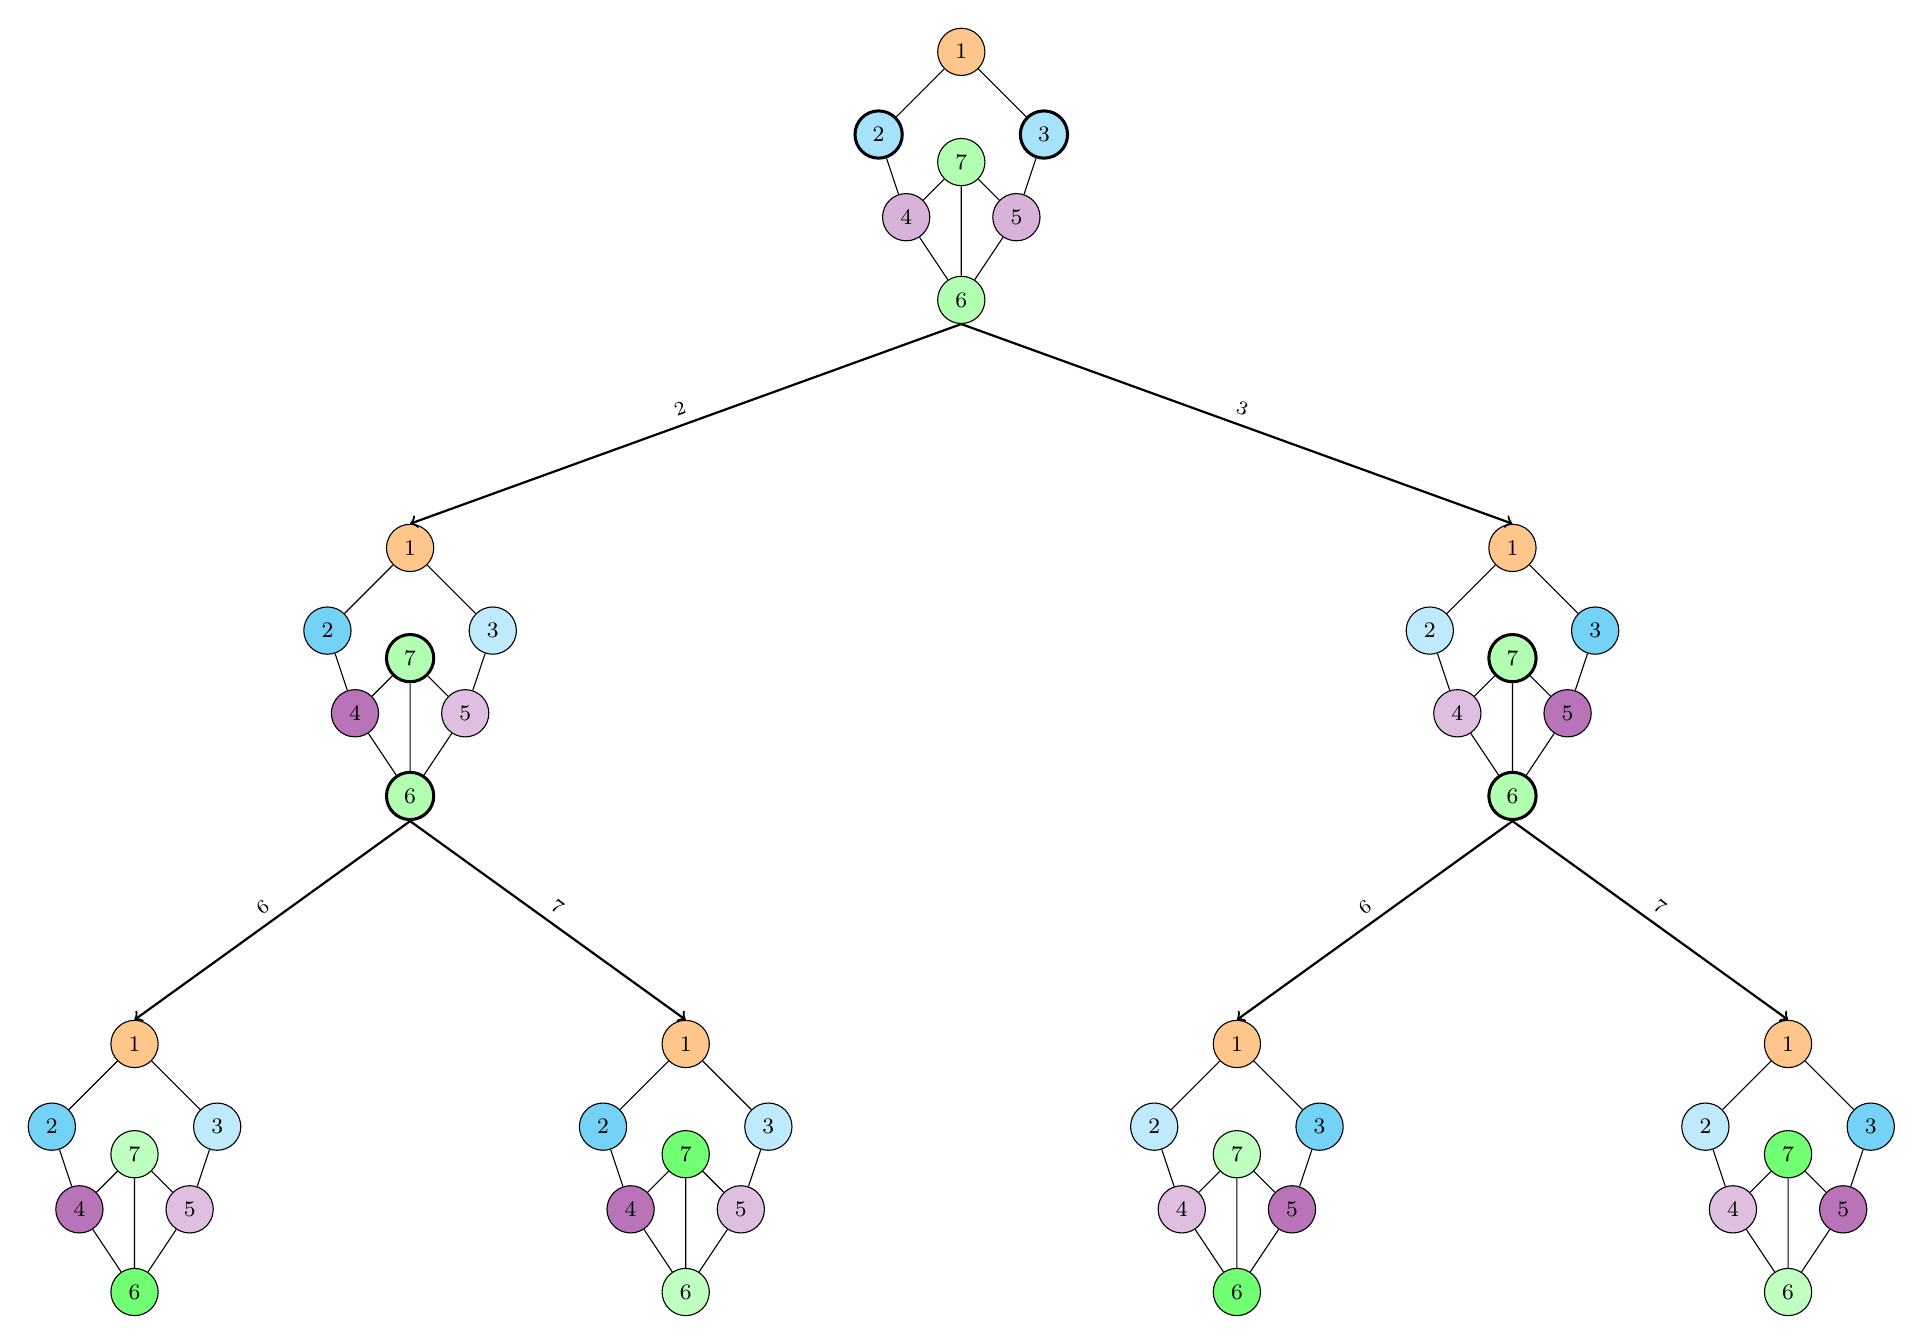
\begin{tikzpicture}[scale=0.7]

    \tikzset{
        v/.style={
            circle,
            draw,
            minimum size=6mm,
            inner sep=0pt,
            font=\footnotesize
        },
        vt/.style={
            v,
            line width=1.1pt
        }
    }

    % ============================================================
    % Niveau 0 : racine
    % ============================================================
    \begin{scope}[xshift=0cm, yshift=0cm]

        \node[v, fill=orange!45] (r1) at (0,2.5) {1};
        \node[vt, fill=cyan!35] (r2) at (-1.5,1) {2};
        \node[vt, fill=cyan!35] (r3) at (1.5,1) {3};
        \node[v, fill=violet!30] (r4) at (-1,-0.5) {4};
        \node[v, fill=violet!30] (r5) at (1,-0.5) {5};
        \node[v, fill=green!30] (r6) at (0,-2) {6};
        \node[v, fill=green!30] (r7) at (0,0.5) {7};

        \draw
            (r1)--(r2)
            (r1)--(r3)
            (r2)--(r4)
            (r3)--(r5)
            (r4)--(r6)
            (r5)--(r6)
            (r4)--(r7)
            (r5)--(r7)
            (r6)--(r7);

    \end{scope}


    % ============================================================
    % Niveau 1 gauche : individualisation de 2
    % ============================================================
    \begin{scope}[xshift=-10cm, yshift=-9cm]

        \node[v, fill=orange!45] (l1) at (0,2.5) {1};
        \node[v, fill=cyan!55] (l2) at (-1.5,1) {2};
        \node[v, fill=cyan!25] (l3) at (1.5,1) {3};
        \node[v, fill=violet!55] (l4) at (-1,-0.5) {4};
        \node[v, fill=violet!25] (l5) at (1,-0.5) {5};
        \node[vt, fill=green!30] (l6) at (0,-2) {6};
        \node[vt, fill=green!30] (l7) at (0,0.5) {7};

        \draw
            (l1)--(l2)
            (l1)--(l3)
            (l2)--(l4)
            (l3)--(l5)
            (l4)--(l6)
            (l5)--(l6)
            (l4)--(l7)
            (l5)--(l7)
            (l6)--(l7);

    \end{scope}


    % ============================================================
    % Niveau 1 droite : individualisation de 3
    % ============================================================
    \begin{scope}[xshift=10cm, yshift=-9cm]

        \node[v, fill=orange!45] (s1) at (0,2.5) {1};
        \node[v, fill=cyan!25] (s2) at (-1.5,1) {2};
        \node[v, fill=cyan!55] (s3) at (1.5,1) {3};
        \node[v, fill=violet!25] (s4) at (-1,-0.5) {4};
        \node[v, fill=violet!55] (s5) at (1,-0.5) {5};
        \node[vt, fill=green!30] (s6) at (0,-2) {6};
        \node[vt, fill=green!30] (s7) at (0,0.5) {7};

        \draw
            (s1)--(s2)
            (s1)--(s3)
            (s2)--(s4)
            (s3)--(s5)
            (s4)--(s6)
            (s5)--(s6)
            (s4)--(s7)
            (s5)--(s7)
            (s6)--(s7);

    \end{scope}


    % ============================================================
    % Niveau 2 :  2 ->  6
    % ============================================================
    \begin{scope}[xshift=-15cm, yshift=-18cm]

        \node[v, fill=orange!45] (a1) at (0,2.5) {1};
        \node[v, fill=cyan!55] (a2) at (-1.5,1) {2};
        \node[v, fill=cyan!25] (a3) at (1.5,1) {3};
        \node[v, fill=violet!55] (a4) at (-1,-0.5) {4};
        \node[v, fill=violet!25] (a5) at (1,-0.5) {5};
        \node[v, fill=green!55] (a6) at (0,-2) {6};
        \node[v, fill=green!25] (a7) at (0,0.5) {7};

        \draw
            (a1)--(a2)
            (a1)--(a3)
            (a2)--(a4)
            (a3)--(a5)
            (a4)--(a6)
            (a5)--(a6)
            (a4)--(a7)
            (a5)--(a7)
            (a6)--(a7);

    \end{scope}


    % ============================================================
    % Niveau 2 :  2 ->  7
    % ============================================================
    \begin{scope}[xshift=-5cm, yshift=-18cm]

        \node[v, fill=orange!45] (b1) at (0,2.5) {1};
        \node[v, fill=cyan!55] (b2) at (-1.5,1) {2};
        \node[v, fill=cyan!25] (b3) at (1.5,1) {3};
        \node[v, fill=violet!55] (b4) at (-1,-0.5) {4};
        \node[v, fill=violet!25] (b5) at (1,-0.5) {5};
        \node[v, fill=green!25] (b6) at (0,-2) {6};
        \node[v, fill=green!55] (b7) at (0,0.5) {7};

        \draw
            (b1)--(b2)
            (b1)--(b3)
            (b2)--(b4)
            (b3)--(b5)
            (b4)--(b6)
            (b5)--(b6)
            (b4)--(b7)
            (b5)--(b7)
            (b6)--(b7);

    \end{scope}


    % ============================================================
    % Niveau 2 :  3 ->  6
    % ============================================================
    \begin{scope}[xshift=5cm, yshift=-18cm]

        \node[v, fill=orange!45] (c1) at (0,2.5) {1};
        \node[v, fill=cyan!25] (c2) at (-1.5,1) {2};
        \node[v, fill=cyan!55] (c3) at (1.5,1) {3};
        \node[v, fill=violet!25] (c4) at (-1,-0.5) {4};
        \node[v, fill=violet!55] (c5) at (1,-0.5) {5};
        \node[v, fill=green!55] (c6) at (0,-2) {6};
        \node[v, fill=green!25] (c7) at (0,0.5) {7};

        \draw
            (c1)--(c2)
            (c1)--(c3)
            (c2)--(c4)
            (c3)--(c5)
            (c4)--(c6)
            (c5)--(c6)
            (c4)--(c7)
            (c5)--(c7)
            (c6)--(c7);

    \end{scope}


    % ============================================================
    % Niveau 2 :  3 ->  7
    % ============================================================
    \begin{scope}[xshift=15cm, yshift=-18cm]

        \node[v, fill=orange!45] (d1) at (0,2.5) {1};
        \node[v, fill=cyan!25] (d2) at (-1.5,1) {2};
        \node[v, fill=cyan!55] (d3) at (1.5,1) {3};
        \node[v, fill=violet!25] (d4) at (-1,-0.5) {4};
        \node[v, fill=violet!55] (d5) at (1,-0.5) {5};
        \node[v, fill=green!25] (d6) at (0,-2) {6};
        \node[v, fill=green!55] (d7) at (0,0.5) {7};

        \draw
            (d1)--(d2)
            (d1)--(d3)
            (d2)--(d4)
            (d3)--(d5)
            (d4)--(d6)
            (d5)--(d6)
            (d4)--(d7)
            (d5)--(d7)
            (d6)--(d7);

    \end{scope}


    % ============================================================
    % Flèches niveau 0 -> niveau 1
    % ============================================================

    \draw[->, thick]
        (r6.south)
        -- node[midway, above, sloped, font=\scriptsize] { $2$}
        (l1.north);

    \draw[->, thick]
        (r6.south)
        -- node[midway, above, sloped, font=\scriptsize] { $3$}
        (s1.north);


    % ============================================================
    % Flèches niveau 1 gauche -> niveau 2
    % ============================================================

    \draw[->, thick]
        (l6.south)
        -- node[midway, above, sloped, font=\scriptsize] { $6$}
        (a1.north);

    \draw[->, thick]
        (l6.south)
        -- node[midway, above, sloped, font=\scriptsize] { $7$}
        (b1.north);


    % ============================================================
    % Flèches niveau 1 droite -> niveau 2
    % ============================================================

    \draw[->, thick]
        (s6.south)
        -- node[midway, above, sloped, font=\scriptsize] { $6$}
        (c1.north);

    \draw[->, thick]
        (s6.south)
        -- node[midway, above, sloped, font=\scriptsize] { $7$}
        (d1.north);

\end{tikzpicture}